\documentclass{beamer}
\usepackage[utf8]{inputenc} 
\usepackage[russian]{babel} 
\newenvironment{compactlist}{
    \begin{list}{{$\bullet$}}{
      \setlength\partopsep{0pt}
      \setlength\parskip{0pt}
      \setlength\parsep{0pt}
      \setlength\topsep{0pt}
      \setlength\itemsep{0pt}
} }{
\end{list} }
\begin{document}
	\title{Оптимизация стратегии развития программных продуктов с учетом возможностей открытого программного обеспечения}   
	\author{Черкашин Дмитрий} 
	\date{\today} 
	
	
	\frame{\titlepage
	\begin{center}
		Научный руководитель -- Смирнов А.И.
	\end{center}
	}
	
	\frame{\frametitle{Содержание}\tableofcontents}
	\section{Введение}
	\frame{\frametitle{Введение}
		Следует ли открывать часть исходного кода своего ПО, что бы задействовать таланты добровольцев в разработке за пределами фирмы, в обмен на предоставление этого ПО бесплатно?
	}
	\section{Построение модели}
	\frame{ 
		\frametitle{Построение модели. ЗИК}
	$K(t)$ -- Качество продукта

	$\nu (t) \ge 0$  -- Инвестиции в продукт, $\nu(t)' > 0$, $\nu(t)'' < 0$
	
	$\dot K(t) = h(\nu) - \delta K$ --  развитие уровня качества с течением времени для ЗИК, $\delta K$ отражает <<устаревание>> продукта.

	$p_s(t) \ge 0$ -- цена основного продукта

	$p_a(t) \ge 0$ -- цена дополнительного продукта

	$\beta$ - коэффициент $R \& D$ затрат

	$r$ -- ставка дисконтирования

	$\phi$ -- влияние изменения цены на ОП

	$q_s = K - \phi p_s$ -- спрос на ОП, $\phi$ -- влияние изменения цены на качество ОП

	$q_a = (\alpha - p_a)q_s$ -- спрос на ДП, $\alpha$ -- коэффициент влияния цены ДП на его качество

	$\max_{p_s, p_a, \nu \ge 0} \int_0^{\infty} e^{-rt}(p_s q_s + p_a q_a - \beta \nu) dt$ -- прибыль для ОИК
	}



	\frame{ 
		\frametitle{Построение модели. ОИК}
	$g(q_s)$ -- вклад общества в качество программного обеспечения, $g(q_s)' > 0$, $g(q_s)'' < 0$.

	$\dot K(t) = h(\nu) + g(q_s) - \delta K$ --  развитие уровня качества с течением времени для ОИК

	$\max_{p_a, \nu \ge 0} \int_0^{\infty} e^{-rt}(p_a q_a - \beta \nu) dt$ -- прибыль для ОИК
	}








	\section{Модель монополиста с отложенным принятием решения}
	\frame{\frametitle{Полученная модель монополиста с отложенным принятием решения} 
	$$
	\left\{
	\begin{aligned}
	& \max_{p_a, \nu \ge 0} (\int_0^{\tau} e^{-rt}(p_s q_s + p_a q_a - \beta \nu) dt + \int_{\tau}^{\infty} e^{-rt}(p_a q_a - \beta \nu) dt )\\
	& \dot K(t) = h(\nu) - \delta K, \  0 \le t < \tau\\
	& \dot K(t) = h(\nu) + g(q_s) - \delta K, \  \tau < t \le \infty\\
	& K(0) = K_0\\
	& p_s = 0, \ \tau < t \le \infty
	\end{aligned}
	\right.
	$$
	}
	
	\section{Анализ модели}
	\frame{\frametitle{Оптимальное управление для ЗИК}
	$$
	\left\{
	\begin{aligned}
	&p_s^{*} =
	\left\{ 
	\begin{aligned}
	  &\frac{1}{2} \left( \frac{K}{\phi} - \frac{\alpha^2}{4} \right), K > \frac{\alpha^2\phi}{4}\\
	  &0, K \le \frac{\alpha^2\phi}{4}
	\end{aligned}
	\right.
	, \\
	& p_a^* = \frac{\alpha}{2},\\  
	& \nu^* = \left( \frac{ab\psi}{\beta} \right)^{\frac{1}{1-b}}\\
	\end{aligned}
	\right.
	$$
	}

	\frame{\frametitle{Оптимальное управление для ЗИК}
	$$
	\left\{
	\begin{aligned}
	& p_s^* = 0 \\
	& p_a^* = \frac{\alpha}{2},  \\ 
	& \nu^* = \left( \frac{ab\psi}{\beta} \right)^{\frac{1}{1-b}} 
	\end{aligned}
	\right.
	$$
	}
	

	\frame{\frametitle{Параметры для подстчетов}
	$$	
	\begin{tabular}{|r|r|r|r|r|r|r|r|}
	\hline
	r & $\alpha$ & $\phi$ & $\beta$ & a & b & m & n \\
	\hline
	0.1 & 5 & 5 & 0.05 & 1 & 0.5 & 0.25 & 0.5\\
	\hline
	\end{tabular}
	$$
	}

	\section{Выводы}

	\frame{\frametitle{Выводы}
		1. Если затраты на $R\&D$ низки, либо фирма должна сразу перевести ОП на ОИК, либо навсегда остаться на ЗИК.
	
		2. Если затраты на $R\&D$ высоки, то всегда оптимально открыть исходный код.
		
		3. Для средних затрат на $R\&D$  решения о том, следует ли открывать исходный код, время открытия оного, зависят от начального качества продукта.
	}

	\frame{\frametitle{Выводы}
		4. Пренебрежение возможностью создания программного обеспечения с открытым исходным кодом в определенное оптимальное время $\tau^*$ означает потерю прибыли; это упущение достигает максимума в тех точках, где оба варианта (навсегда остаться на ЗИК или моментально перейти на ОИК) одинаково выгодны.
	}

	\frame{\frametitle{Выводы}
		5. Если в какое-то оптимально определенное время вы не включаете опцию открытия программного обеспечения с открытым исходным кодом, оптимально сделать программное обеспечение с открытым исходным кодом более высокого качества. Эта разница в качестве, при которой открывается исходный код, увеличивается за счет затрат на $R\&D$.
	}
	
	\frame{\frametitle{Выводы}	
		6. Чем больше исходное качество, тем позднее фирма откроет свой исходный код.
		

		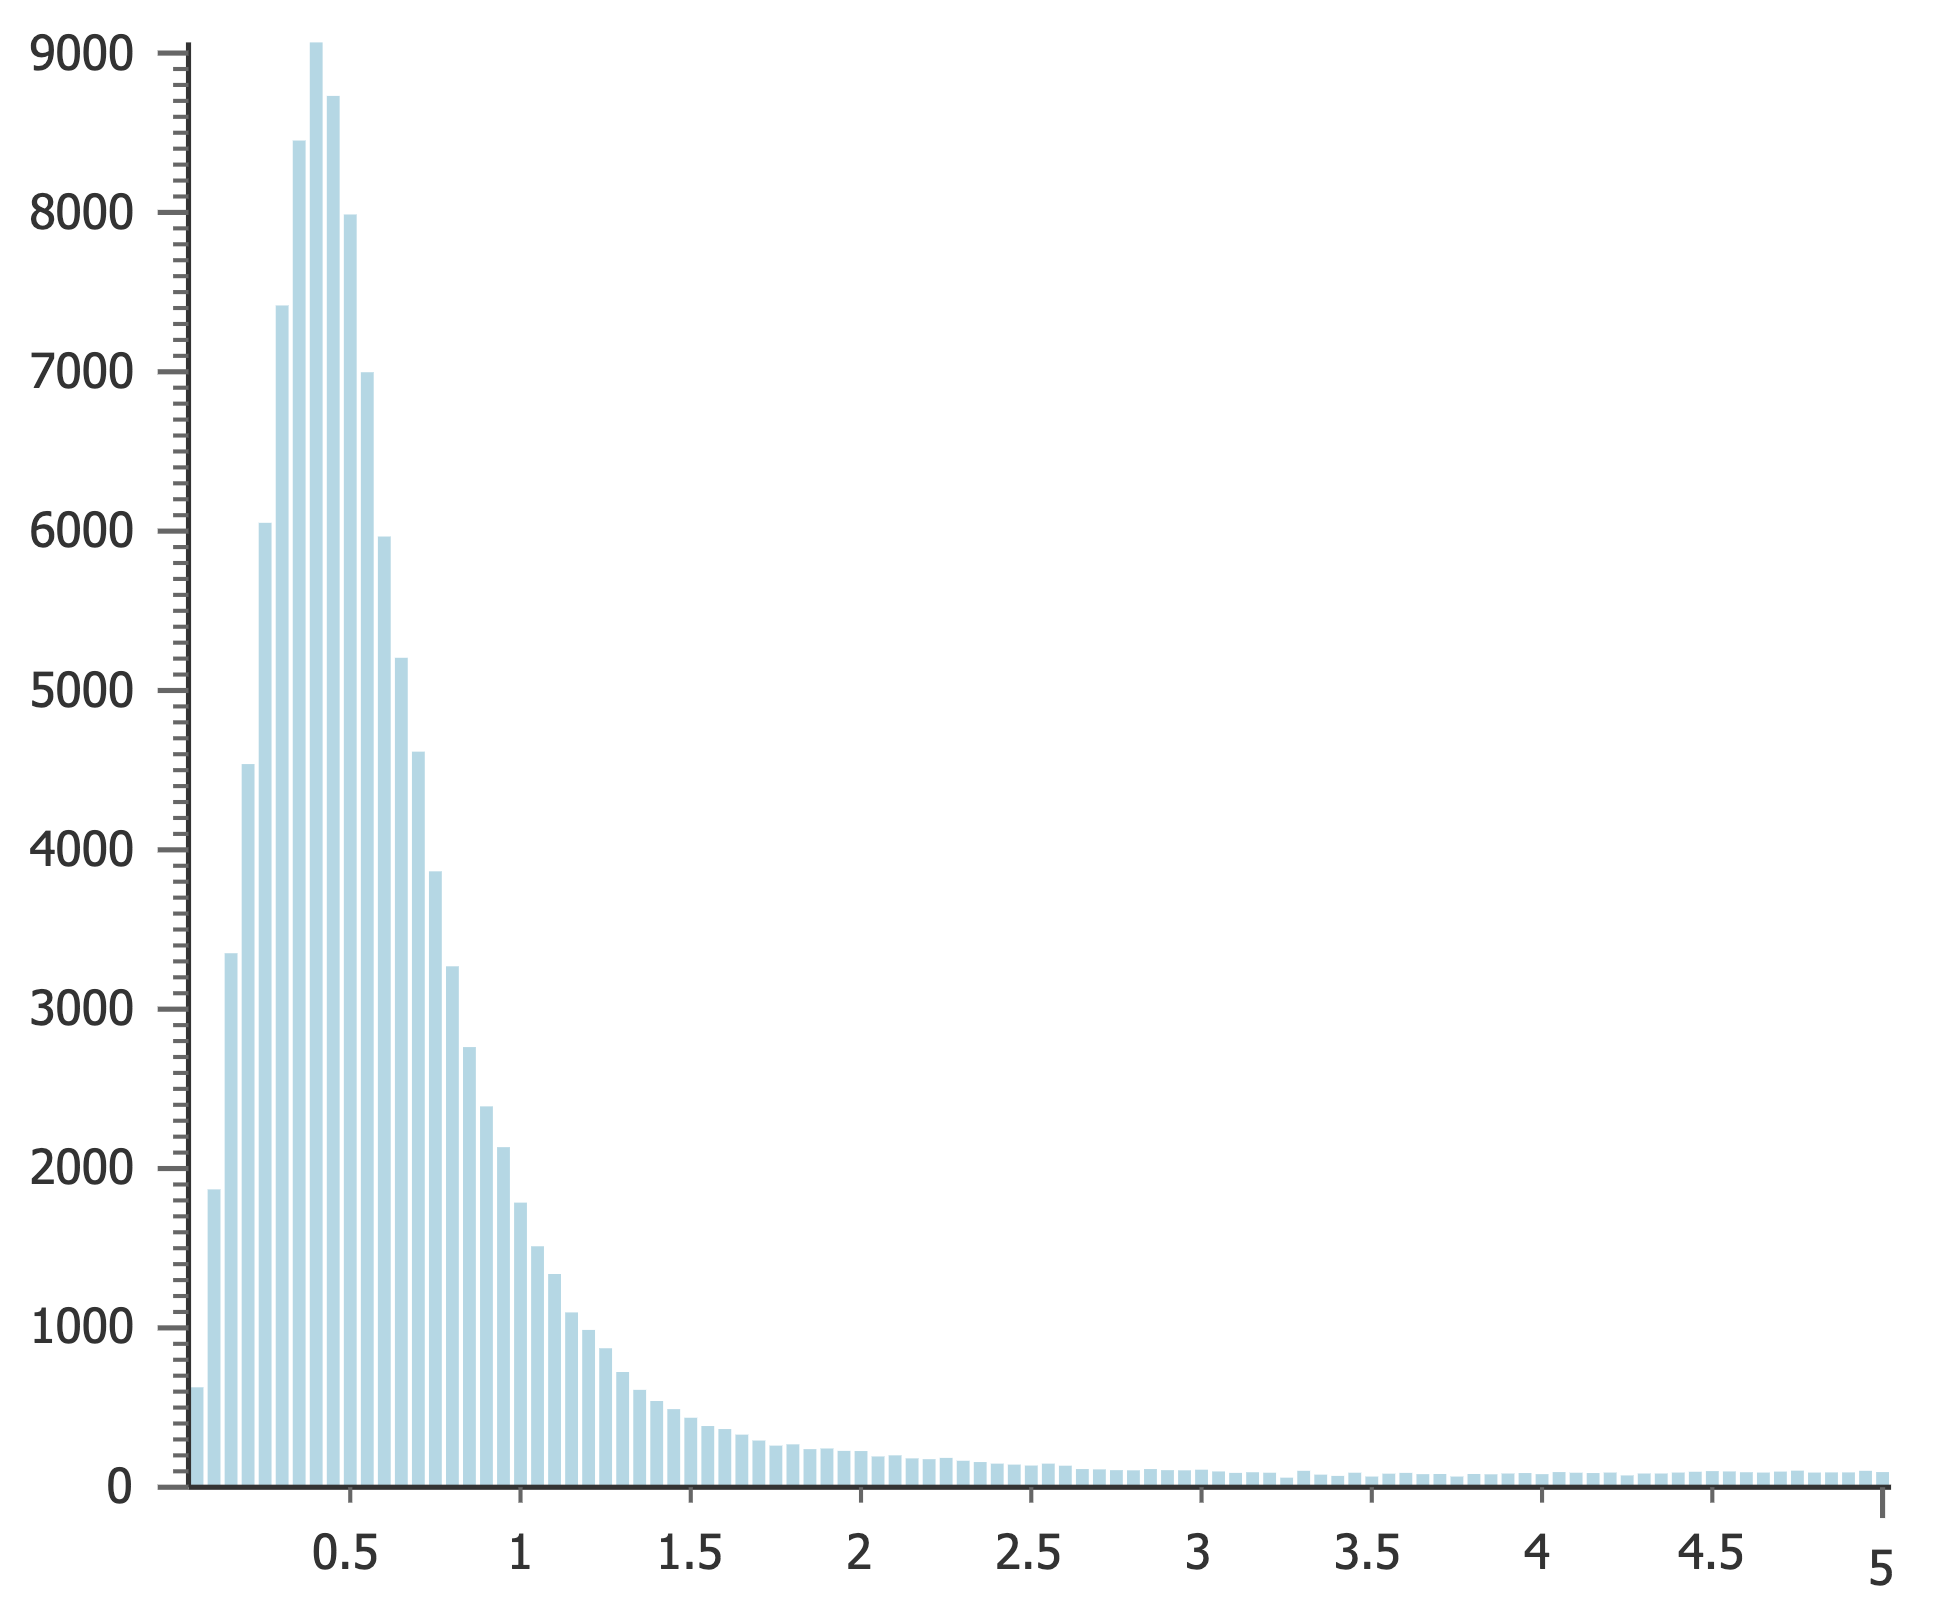
\includegraphics[width=10.8cm, height=5.06cm]{lol}

	}

	\frame{\frametitle{Выводы}
	
		7. Увеличение параметров $m, \alpha, \beta, \delta, \phi$ уменьшает оптимальное время переключения, в то время как $a$  увеличивает это время.}
	
	\frame{\frametitle{Список Литературы}
		\begin{enumerate}
		\item \textit{Haruvy, Sethi, and Zhou} Open Source Development with a Commercial Complementary Product or Service // Production and Operations Management 17(1), 2008. С. 29. — 43.
		\item \textit{Caulkins, J.P., Feichtinger, G., Grass, D., Hartl, R.F., Kort, P.M., Seidl, A.}  When to make proprietary software open source. // Journal of Economic Dynamics and Control 37, 2013. 1182. — 1194.
		\item \textit{Makris, M.} Necessary conditions for infinite-horizon discounted two-stage optimal control problems. // Journal of Economic Dynamics and Control 25 (12), 2001. 1935–1950.
		\end{enumerate}
		}
		\end{document}
